
%%%%%%%%%%%%%%%%%%%%%%%%%%%%%%%%%%%%%%%%%%%%%%%%%%%%%%%%
%
% Copyright (c) 2003-2009 by University of Queensland
% Earth Systems Science Computational Center (ESSCC)
% http://www.uq.edu.au/esscc
%
% Primary Business: Queensland, Australia
% Licensed under the Open Software License version 3.0
% http://www.opensource.org/licenses/osl-3.0.php
%
%%%%%%%%%%%%%%%%%%%%%%%%%%%%%%%%%%%%%%%%%%%%%%%%%%%%%%%%

\section{Two Dimensional Heat Diffusion for a basic Magmatic Intrusion}
\sslist{twodheatdiff001.py and cblib.py}
\label{Sec:2DHD}
 Building upon our success from the 1D models, it is now prudent to expand our domain by another dimension. For this example we will be using a very simple magmatic intrusion as the basis for our model. The simulation will be a single event where some molten granite has formed a hemispherical dome at the base of some cold sandstone country rock. A hemisphere is symmetric so taking a cross-section through its centre will effectively model a 3D problem in 2D. New concepts will include non-linear boundaries and the ability to prescribe location specific variables.

\begin{figure}[h!]
\centerline{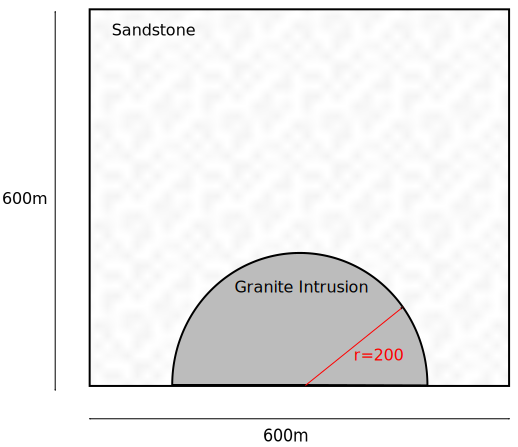
\includegraphics[width=4.in]{figures/twodheatdiff}}
\caption{2D model: granitic intrusion of sandstone country rock.}
\label{fig:twodhdmodel}
\end{figure}

To expand upon our 1D problem, the domain must first be expanded. This will be done in our definition phase by creating a square domain in $x$ and $y$ that is 600 meters along each side \reffig{fig:twodhdmodel}. The number of discrete spatial cells will be 100 in either direction. The radius of the intrusion will be 200 meters with the centre located at the 300 meter mark on the x-axis. The domain variables are;
\begin{python}
mx = 600*m #meters - model length
my = 600*m #meters - model width
ndx = 100 #mesh steps in x direction 
ndy = 100 #mesh steps in y direction
r = 200*m #meters - radius of intrusion
ic = [300, 0] #centre of intrusion (meters)
q=0.*Celsius #our heat source temperature is now zero
\end{python}
The next step is to define our variables for each material in the model in a manner similar to the previous tutorial. Note that each material has its own unique set of values. The time steps and set up for the domain remain as in Section \ref{sec:key}. Prior to setting up the PDE the boundary between the two materials must be established. The distance $s$ between two points in Cartesian coordinates is defined as:
\begin{equation}
 (x_{1}-x_{0})^{2}+(y_{1}-y_{0})^{2} = s^{2}
\end{equation}
If we define the point $[x_{0},y_{0}]$ as $c$ which denotes the centre of the semi-circle of our intrusion, then for all the points $[x,y]$ in our model we can calculate a distance to $c$. All the points that fall within the radius $r$ of our intrusion will have a corresponding value $s < r$ and all those belonging to the country rock will have a value $s > r$. By subtracting $r$ from both of these conditions we find $s-r < 0$ for all intrusion points and $s-r > 0$ for all country rock points. Defining these conditions within the script is quite simple and is done using the following command:
\begin{python}
 bound = length(x-ic)-r #where the boundary will be located
\end{python}
This definition of the boundary can now be used with the \verb wherePositive()  and \verb whereNegative()  commands to help define the material constants and temperatures in our domain. By examining the general form we solved in the earlier tutorials, it is obvious that both \verb A  and \verb D  depend on the predefined variables. To set these variables accordingly and complete our PDE we use:
\begin{python}
A = (kappai)*whereNegative(bound)+(kappac)*wherePositive(bound)
D = (rhocpi/h)*whereNegative(bound)+(rhocpc/h)*wherePositive(bound)

mypde.setValue(A=A*kronecker(model),D=D,d=eta,y=eta*Tc)
\end{python}
Our PDE has now been properly established. The initial conditions for temperature are set out in a similar matter:
\begin{python}
#defining the initial temperatures.
 T= Ti*whereNegative(bound)+Tc*wherePositive(bound) 
\end{python}
The iteration process now begins as before, but using our new conditions for \verb D  as defined above.

\subsection{Contouring escript data}
It is possible to contour our solution using \modmpl . Unfortunately the \modmpl contouring function only accepts regularly gridded data. As our solution is not regularly gridded, it is necessary to interpolate our solution onto a regular grid. First we extract the model coordinates using \verb getX  these are then transformed to a \verb numpy  array known as a \verb tuple . Ths multi-dimensional array is then broken down into individual $x$ and $y$ arrays. This is a one step process using the function \verb toXYTuple . We also need to generate our regular grid which is done using the \modnumpy function \verb linspace  . 
\begin{python}
# rearrage mymesh to suit solution function space for contouring      
oldspacecoords=model.getX()
coords=Data(oldspacecoords, T.getFunctionSpace())
coordX, coordY = toXYTuple(coords)
# create regular grid
xi = np.linspace(0.0,mx,100)
yi = np.linspace(0.0,my,100)
\end{python}
The remainder of our contouring commands reside within a \verb while  loop so that a new contour is generated for each time step. For each time step the solution must be regridded for \modmpl using the \verb griddata  function. This function interprets an irregular grid and solution from \verb tempT  , \verb xi   and \verb yi . This is transformed to the new coordinates defined by \verb coordX  and \verb coordY  with an output \verb zi  . It is now possible to use the \verb contourf  function which generates colour filled contours. The colour gradient of our plots is set via the command \verb pl.matplotlib.pyplot.autumn() , other colours are listed on the \modmpl web page. Our results are then contoured, visually adjusted using the \modmpl functions and then saved to file. \verb pl.clf()  clears the figure in readiness for the next time iteration.

\begin{python}
#grid the data.
zi = pl.matplotlib.mlab.griddata(coordX,coordY,tempT,xi,yi)
# contour the gridded data, plotting dots at the randomly spaced data points.
pl.matplotlib.pyplot.autumn()
pl.contourf(xi,yi,zi,10)
CS = pl.contour(xi,yi,zi,5,linewidths=0.5,colors='k')
pl.clabel(CS, inline=1, fontsize=8)
pl.axis([0,600,0,600])
pl.title("Heat diffusion from an intrusion.")
pl.xlabel("Horizontal Displacement (m)")
pl.ylabel("Depth (m)")
pl.savefig(os.path.join(save_path,"heatrefraction%03d.png") %i)
pl.clf()        
\end{python}

\begin{figure}[h!]
\centerline{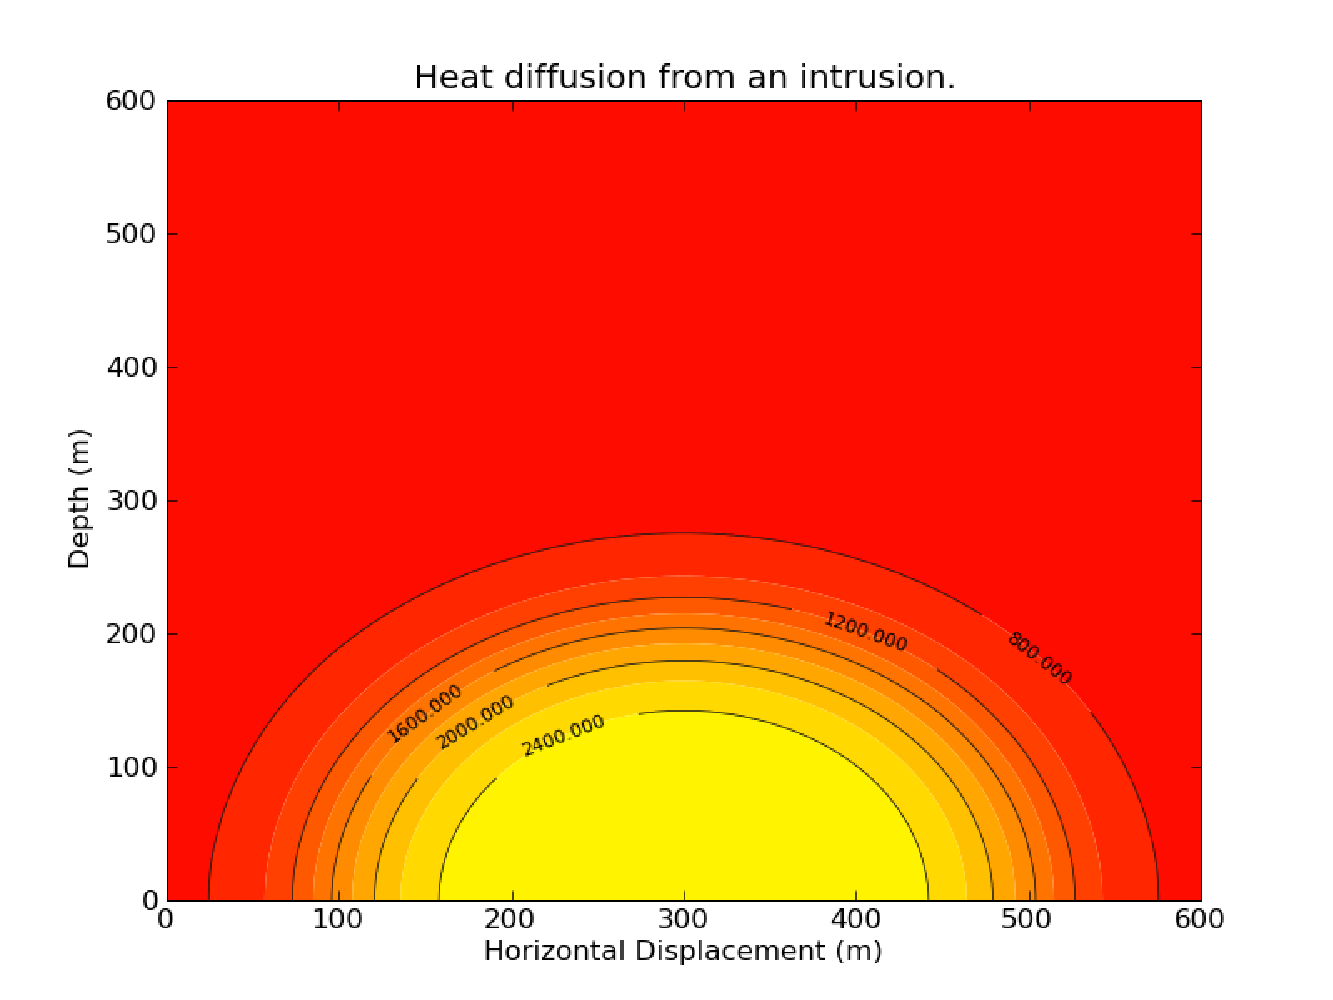
\includegraphics[width=4.in]{figures/heatrefraction050}}
\caption{2D model: Total temperature distribution ($T$) at time $t=50$.}
\label{fig:twodhdans}
\end{figure}

\subsection{Advanced Visualization using VTK}

\subsubsection{Parallel scripts (MPI)}
In some of the example files for this cookbook the plotting commands are a little different.
For example,
\begin{python}
	if getMPIRankWorld() == 0:
	    pl.savefig(os.path.join(save_path+"/totT","ttrodpyplot%03d.png")%i)
	pl.clf()	
\end{python}

The additional \verb if  statement is not necessary for normal desktop use.
It becomes important for scripts run on parallel computers.
Its purpose is to ensure that only one copy of the file is written.
For more details on writing scripts for parallel computing please consult the \emph{user's guide}.